\chapter{System Design II: Behavior Models}
\graphicspath{ {./chapter06/Fig} }

\begin{itquote}
Genius is 1\% inspiration and 99\% perspiration.---Thomas Edison
\end{itquote}


The functional decomposition technique examined in Chapter 5 is a
powerful modeling tool for system design that is applicable for
describing input, output, and transform behavior. However, that approach
by itself is limited in its descriptive ability. This was apparent in
the digital stopwatch example that required the use of state diagrams,
in addition to functional decomposition, to fully articulate the design.
A state diagram is an example of a model, a standardized abstraction of
a system. Models allow systems to be described without having to
determine all of the implementation details. All models are not the
same---they come in a variety of forms and each serves a different
intention.

This chapter provides an overview of other design tools for describing
system behavior, with an emphasis on computing systems. The first tool
examined is the state diagram. This is followed by the flowchart, which
describes algorithmic processes and logical behavior. Two modeling
languages for information and data handling---data flow diagrams and
entity relationship diagrams---are then examined. The final is the
Unified Modeling Language, which is a collection of system views for
describing behavior.

\section*{Learning Objectives}
\noindent\rule{\linewidth}{1pt}
By the end of this chapter, the reader should:

\begin{itemize}
\item
  Be familiar with the following modeling tools for describing system
  behavior: state diagrams, flowcharts, data flow diagrams, entity
  relationship diagrams, and the Unified Modeling Language.
\item
  Understand the intention and expressive power of the different models.
\item
  Understand the domains in which the models apply.
\item
  Be able to conduct analysis and design with the models.
\item
  Understand what model types to choose for a given design problem.
\end{itemize}

\section{Models}
\label{section:models}

From the previous chapter we know that the top-down design process
starts with an abstraction of the system to be built. This initial
design is called an abstraction because it captures the essential
characteristics of the system without specifying the underlying physical
realization. An abstraction that is expressed in a standardized and
accepted language is called a model. In other words a model is a
standardized representation of a system, process, or object which
captures its essential details without specifying the physical
realization. A modeling language does not have to be formed from letters
and words---often the words are graphical symbols. You are already
familiar with many different models from everyday life such as
blueprints, a diagram of a football play, knitting instructions,
electrical schematics, and mathematical formulas to name a few. In order
to be effective, a model should meet the following properties
{[}Sat02{]}:

\begin{itemize}
\item
  \emph{Be abstract.} This means that the model should be independent of
  final implementation and that there should be multiple ways of
  implementing the design based upon it.
\item
  \emph{Be unambiguous.} A model should have a single clear meaning in
  terms of describing the intended behavior.
\item
  \emph{Allow for innovation.} Models should encourage exploration of
  alternative system implementations and behaviors.
\item
  \emph{Be standardized.} Standardization provides a common language
  that can be understood by all. Designers should be wary of developing
  their own models that are ill-defined and not commonly understood.
\item
  \emph{Provide a means for communication.} A model should facilitate
  communication within the design team and with non-technical
  stakeholders.
\item
  \emph{Be modifiable.} A model should make design modifications
  relatively easy.
\item
  \emph{Remove unnecessary details and emphasize important features.}
  The intent is to simplify the design for ease of understanding. The
  most highly detailed information is typically identified in the
  detailed design.
\item
  \emph{Break the overall problem into sub-problems.} Most problems are
  too complex to be handled directly and must be decomposed into
  subsystems. This produces the design hierarchy.
\item
  \emph{Substitute a sequence of actions by a single action.} This
  allows understanding of the overall larger behavior, which can then be
  examined at other levels. This supports the ability to break a design
  into sub-problems.
\item
  \emph{Assist in verification.} A model should aid in demonstrating
  that the design meets the engineering requirements.
\item
  \emph{Assist in validation.} Validation is the process of
  demonstrating that the needs of the user are being met and the right
  system is being designed. The model should facilitate discussion with
  all stakeholders to ensure it meets everyone's expectations.
\end{itemize}

In order to meet these properties, most models have an
\emph{\textbf{object type,}} which is capable of encapsulating the
actual components used to construct the target system. In order to
capture the dependence of objects on one another models typically have a
\emph{\textbf{relationship type}}. Finally, models have an
\emph{\textbf{intention,}} which is the intended class of behavior that
it describes. For example, the intention of a circuit schematic and the
schematic of a football play are entirely different. Since models are
built with different intentions, it possible to choose the wrong model
for a particular system---it would surprise a football team to see a
play represented with resistors and capacitors!

Since models capture the essential details of a system in a standardized
way then they are an ideal way to describe the functionality of a system
at all levels of detail. In Chapter 5 the predominate method of
describing functionality was with words. However, there are languages
that describe system behavior. We start by examining state diagrams.

\section{State Diagrams}
\label{section:state-diagrams}

\emph{\textbf{State diagrams}} describe the behavior of systems with
memory. A system with memory is able to modify its response to inputs
based on the state of the system. The \emph{\textbf{state}} of a system
represents the net effect of all previous inputs to the system. Since
the state characterizes the history of previous inputs, it is often
synonymous with the word memory. Intuitively, a state corresponds to an
operating mode of a system, and inputs are associated with transitions
between states. To determine if a system has memory, ask the following
question--- ``\emph{Can the same input produce different outputs?}'' If
the answer to this question is yes, then the system has memory and can
be modeled with a state diagram.

A state diagram is a drawing that consists of states and transition arcs
as shown in Figure~\ref{figure:stateDiagramSymbols}. 
Each state is represented as a rectangle with
rounded edges with the name of the state written inside. Whenever
possible, states should be given meaningful names. When there exists the
possibility for ambiguity in the names, a table should be created that
identifies the state names and their associated meanings. There are
special circle symbols for both initial and final states. Transitions
are drawn as arrows from a source state to a destination state. Since
inputs cause the transitions between states, the arrows are labeled with
their associated inputs. The outputs are listed directly in the state
since it is assumed that the outputs are associated with states.


\begin{figure}
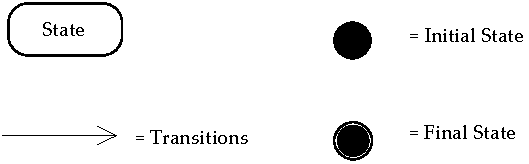
\includegraphics[width=3.28in,height=1in]{./image1}
\caption{Symbols used in state diagrams.}
\label{figure:stateDiagramSymbols}
\end{figure}


As an example, consider a vending machine that accepts nickels and dimes
and dispenses a piece of candy when 25 cents has been deposited. This
vending machine can be modeled using a state diagram because the
response of the machine to a coin depends on how much money has been
deposited so far.

In order to give a more complete description of the vending machine the
state diagram is embedded into the function table template introduce in
Chapter 5as shown in Figure~\ref{table:stateVendingMachine}.
 This table lists the inputs and outputs
of the vending machine along with the behavior represented by a state
diagram.

\begin{table}
\caption{A state diagram for a simple vending machine.}
\label{table:stateVendingMachine}
\begin{tabular}{|l|m{10cm}|}
\hline
\emph{Module} &Vending Machine Control Unit \\ \hline
\emph{Inputs} & 
\begin{itemize}
\item
  Nickel: Signals that a nickel has been deposited.
\item
  Dime: Signals that a dime has been deposited.
\end{itemize} \\ \hline

\emph{Outputs} & 
\begin{itemize}
\item
  Reset: Signals the FSM to return to the Initial/Reset state.
\item
  Vend: Signal to dispense candy.
\end{itemize} \\ \hline
\emph{Functionality} &
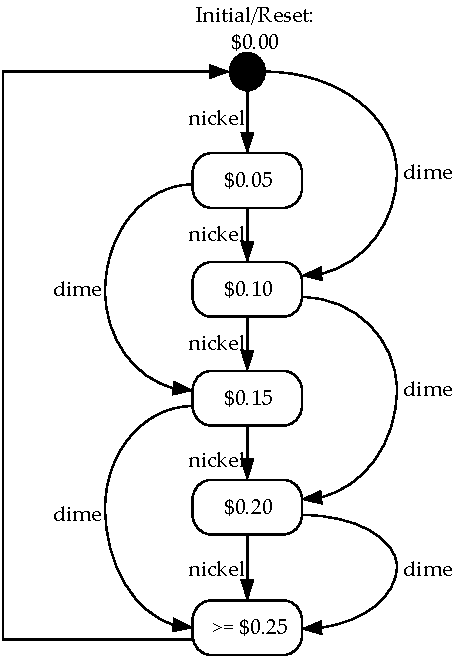
\includegraphics[width=2in,height=3in]{./image2} \\ \hline
\end{tabular}
\end{table}


The initialization/reset state is labeled \$0.00, while the action of
the machine (dispense or not dispense candy) is associated with the
states---the only state that dispenses candy is \$0.25. There are three
types of transitions shown in this state diagram. The two labeled nickel
and dime are associated with depositing those coins. The unlabeled
transition from state \$0.25 to state \$0.00 is called an unconditional
transition. A system with an unconditional transition between two states
is assumed to remain in the first state for a defined time period before
automatically moving to the second state. In this case it ensures that
the machine dispenses a single candy before going on to the next
transaction. It is common practice in state diagrams to assume that any
unspecified input conditions cause the system to remain in the current
state. For example, if no coin is inserted while in state \$0.20 the
system remains in state \$0.20. Finally, note that since this machine
does not dispense change, it can overcharge a customer for candy. This
would not be a popular vending machine with users!

\section{Flowcharts}
\label{section:flowcharts}

The intention of a \emph{\textbf{flowchart}} is to visually describe a
process or algorithm, including its steps and control. Flowcharts are
often scoffed at as being old-fashioned and overly simple---these
criticisms are actually strengths. Since flowcharts have been around for
a long time, they are easily recognized and understood. Furthermore,
being simple makes them accessible to a wide audience. Due to their
simplicity, they are applied in a great number of applications,
including non-technical ones such as the description of business
processes.

Some of the primary symbols used in flowcharts are shown in 
Figure~\ref{figure:basicFlowChartSymbols}.
The names of the starting and ending steps of a flowchart are
represented by ovals known as terminators. Individual processing steps
are written inside of rectangles, while a process step that is
elaborated by another flowchart is drawn as a rectangle with double
sides. Elaborated processes allow the representation of hierarchy in the
design. Certain points in a flowchart can lead to alternative
destinations as represented by a decision or conditional symbol
(diamond). The condition that determines the next step is written inside
the diamond and the possible values of the condition are written on the
arcs leaving the conditional step. As shown in 
Figure~\ref{figure:basicFlowChartSymbols} there are
multiple ways to indicate data stores for retrieving or saving data.

\begin{figure}
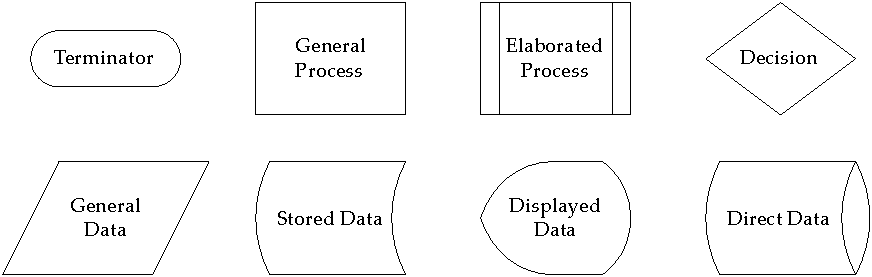
\includegraphics[width=4.9in,height=1.56in]{./image3}
\caption{Basic flowchart symbols.}
\label{figure:basicFlowChartSymbols}
\end{figure}

As an application, consider an embedded computer system that monitors
the light level of its environment as described by the flowchart in
Figure~\ref{table:flowchartEmbedded}. 
The algorithmic process of the flowchart is easy and
intuitive to understand. The system reads the current light value,
stores it into an array, and then computes an average. In a complete
system description, there would be a second flowchart describing how the
system determines the average of the values of the light samples, since
this is identified as an elaborated process. The system then waits 1ms,
writes the average to a terminal (display device), and then checks for a
key-press. Light levels continue to be monitored in the absence of a
key-press, otherwise the light monitoring process halts.


\begin{table}
\caption{A flowchart for an embedded system.}
\label{table:flowchartEmbedded}
\begin{tabular}{|l|m{10cm}|}
\hline

\emph{Module} & Light level data logger \\ \hline
\emph{Inputs} & 
\begin{itemize}
\item
  Light intensity: Ambient light intensity from environment.
\item
  Key-press: User request to abort data logging.
\end{itemize}\\ \hline

\emph{Outputs} & 
\begin{itemize}
\item
  Terminal: Displays the average light intensity.
\item
  Disk: Stores a record of light intensities through time.
\end{itemize} \\ \hline
\emph{Functionality} &
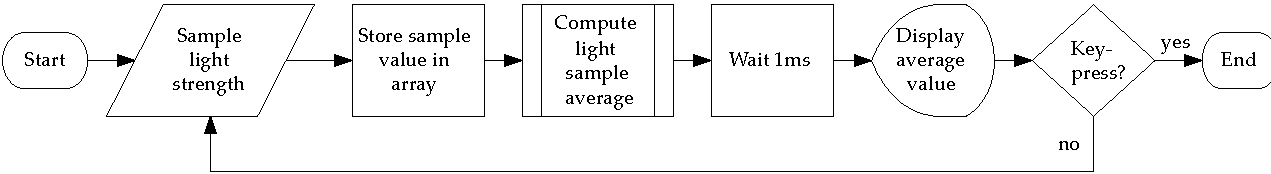
\includegraphics[width=4.7in,height=0.74in]{./image4} \\ \hline
\end{tabular}
\end{table}

\textbf{Figure 6.4} 

Flowcharts are an intuitive way to describe algorithmic processes.
Limiting the complexity of a flowchart to between 10 and 20 steps
enables the sequence of actions to be quickly comprehended while
eliminating unnecessary details. Flowcharts are not able to represent
the structure of data being manipulated and they are not particularly
good at representing concurrent processes. For this we need data flow
diagrams.

\section{Data Flow Diagrams}
\label{section:data-flow-diagrams}

The intention of a \emph{\textbf{data flow diagram}} (DFD) is to model
the processing and flow of data inside a system. It is a
function-oriented approach that is similar to functional
decomposition---the processes inside a DFD accept data inputs, transform
them in some way, and produce output data. A DFD is often used for the
analysis of information systems due to its data emphasis, but can be
broadly applied to ECE systems. It differs from functional decomposition
in that functional decomposition is often closer to the implementation
of the design, whereas the DFD models the system from a data point of
view. A DFD is fundamentally different from a flowchart in that it does
not encapsulate control and sequencing information, but allows multiple
processes running concurrently. There are four symbols, shown in 
Figure~\ref{figure:dataFlowSymbols}, that are used in a DFD:

\begin{enumerate}
\def\labelenumi{\arabic{enumi}.}
\item
  \emph{Processes.} A rectangle with rounded corners that describes a
  useful task or function. They perform a transformation on the data.
\item
  \emph{Data flows.} An arrow representing a data relationship between
  two processes.
\item
  \emph{Data stores.} An open rectangle representing a data repository.
\item
  \emph{Interfaces.} A square describing external agents or entities
  that use the system. They are also referred to as sources and sinks.
\end{enumerate}


\begin{figure}
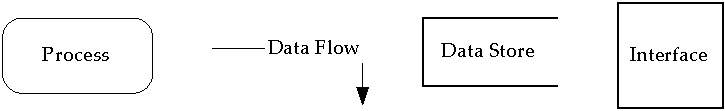
\includegraphics[width=4.6in,height=0.71in]{./image5}
\caption{Data flow diagram symbols.}
\label{figure:dataFlowSymbols}
\end{figure}


Like the general design process, DFDs are successively refined from the
top-down. That is, there is a single top level (or Level 0) DFD
describing the entire system and the interfaces and data stores that it
interacts with. The rules for constructing a DFD are fairly intuitive. A
process must have at least one input and one output. The refinement of a
process at level N must have the same inputs and outputs as the process
at level N-1. Data must be transformed in some way by a process. This
process of refinement continues until a satisfactory level of detail is
reached.

An example of a Level 1 DFD for a video browsing system is shown in
Figure~\ref{table:dataflowVideoBrowse}. Video databases are typically 
very large; due to their size,
it is usually cumbersome to preview videos and extract important
information. A solution to this problem is to apply image analysis
techniques to identify shots (continuous scenes without a break) in a
video and store both the location of the shot boundaries in the video
and key frames that summarize each shot. The collection of key frames is
known as a storyboard. The storyboards are stored in an annotation
database that is much smaller in size than the original video database.
Typically the user of a video browsing system has the ability to preview
the storyboard and select shots from it to view. This example shows the
data flow for such a system.

The data processing is readily apparent from the DFD. Videos in the
database are processed to extract shot boundaries and key frames, which
are stored in the annotation database. The user can submit requests to
view a storyboard, which is retrieved from the annotation database. When
a shot is selected from the storyboard, the users can preview the
original shot, which is retrieved from the video database.

\begin{table}
\caption{Level 1 data flow diagram for a video browsing system.}
\label{table:dataflowVideoBrowse}
\begin{tabular}{|l|m{10cm}|}
\hline
\emph{Module} & Video Browsing System \\ \hline

\emph{Inputs} & 
\begin{itemize}
\item
  Video: External video to the system that is entered into the video
  database.
\item
  Browse Request: User request to browse a particular video.
\item
  Shot Preview Request: User request to preview a particular short from
  a video.
\end{itemize}  \\ \hline
\emph{Outputs} & 
\begin{itemize}
\item
  Story Board: A sequence of frames summarizing the entire video.
\item
  Shot: The complete video corresponding to the still image in the story
  board.
\end{itemize}\\ \hline
\emph{Functionality} &
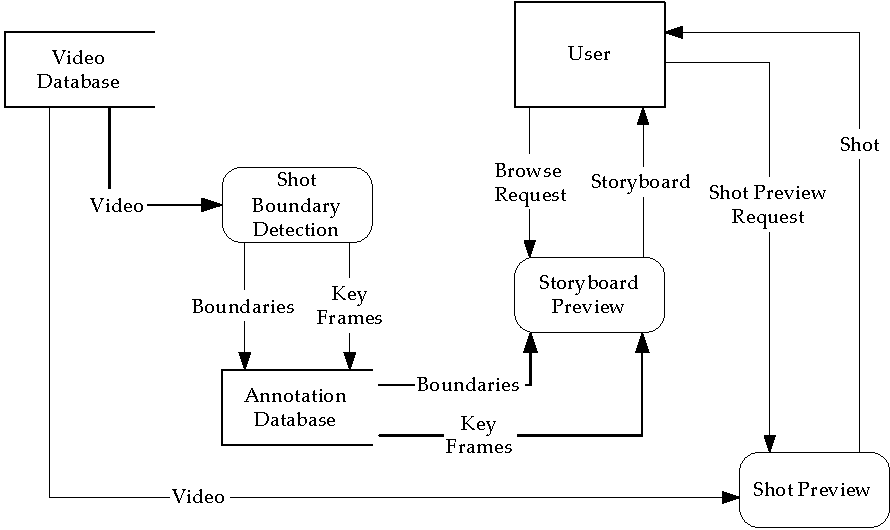
\includegraphics[width=4.9in,height=3.15in]{./image6} \\
\end{tabular}
\end{table}

There are a few important points to note about DFDs. They are solution
independent, specifying the behavior based upon data flow. Specific
information on the data flows is defined in a formal language known as a
\emph{\textbf{data dictionary}} (it is not covered here). There can be
concurrent processes represented in a DFD. In the video browsing
example, multiple people can use the system simultaneously, and there is
no implied sequencing between when the shot boundary detection process
is run and the storyboards are previewed. It is clear that the video
must undergo shot detection prior to viewing its storyboard. This
information is listed in something known as an \emph{\textbf{event
table}}. The event table for this example is shown in Table 6.1.

\textbf{Table 6.1} Event table for the video browsing system.

\begin{table}
\caption{}
\label{table:<context>}
\begin{tabular}{|c|c|c|c|}
\hline
\textbf{Event} & \textbf{Trigger}& \textbf{Process} & \textbf{Source} \\ \hline
Annotate Video & New Video Arrival & Shot Boundary Detection & System \\  \hline
View Storyboard & Browse Request & Storyboard Preview & User \\ \hline
View Shot & Shot Preview Request & Shot Preview & User \\ \hline
\end{tabular}
\end{table}

An \emph{\textbf{event}} is an occurrence at a specific time and place
that needs to be remembered. Events can be classified into temporal,
external, and state. A \emph{temporal event} is one which happens
because the system has reached some critical time. In this example, the
generation of shot boundaries could occur for all new videos in the
database at a specified time each day, but in this case it occurs
whenever a new video is added to the database. An \emph{external event}
occurs outside the system boundary by a system user, in this case
requesting either a storyboard or a video preview. A \emph{state event}
is the result of something changing within the system. Associated with
each event is a \emph{trigger}, the cause of the event. Each event has a
process that is associated with it. Finally, associated with each event
is a \emph{source}, the entity responsible for triggering it.

\section{Entity Relationship Diagrams}
\label{section:entity-relationship-diagrams}

A database is a system that stores and retrieves data, and it is modeled
by an \emph{\textbf{entity relationship diagram}} (ERD). The intention
of an ERD is to catalog a set of related objects (entities), their
attributes, and the relationships between them. The entities and their
relationships are real distinct things that have characteristics that
need to be captured. The design of a database starts by describing the
entities, their attributes, and the relationship between entities in an
ERD. In order to ask meaningful questions about the data, the entities
need to be related to one another. For example, a list of students and a
list of courses by themselves have limited utility. However, by
introducing a relationship between these two entities we can ask
questions such as ``\emph{How many students are taking the
Microelectronics course?}'' The three elements used in the ERD modeling
language are:

\begin{enumerate}
\def\labelenumi{\arabic{enumi}.}
\item
  \emph{Entities.} They are generally in the form of tangible objects,
  roles played, organizational units, devices, and locations. An
  instance is the manifestation of a particular entity. For example, an
  entity could be Student while an instance would be Kristen.
\item
  \emph{Relationships.} They are descriptors for the relationships
  between entities.
\item
  \emph{Attributes.} They are features that are used to differentiate
  between instances of the entities.
\end{enumerate}

Lets consider an ERDs describing academic life at a college . The
process typically starts by interviewing the end-users and identifying
the entities and their attributes. Assume that the result of this
process is that the college wants to store data about three entities:
Students, Courses, and Departments. The process of building an ERD
starts by determining the relationships between entities. One way to do
this is to build an \emph{\textbf{entity relationship matrix}} as shown
in Table~\ref{table:entityRelationshipMatrix}. 
The entities constitute both the row and column headings,
and the matrix entries represent the relationship, if any, that exists
between entities. This is similar to the pairwise comparison matrix in
Chapter 2 where user needs were systematically compared. Relationships
are bi-directional because they have two participating entities.

\begin{table}
\caption{Entity relationship matrix.}
\label{table:entityRelationshipMatrix}
\begin{tabular}{|c|c|c|c|}
\hline
\textbf{Student} & \textbf{Course} & \textbf{Department} \\ \hline
\textbf{Student} & & takes many & majors in one \\ \hline
\textbf{Course} & has many & can require many / can be the prerequisite
for many & is offered by one \\ \hline
\textbf{Department} & enrolls many & offers many & \\ \hline
\end{tabular}
\end{table}

From Table~\ref{table:entityRelationshipMatrix} we can 
see that a Student can take many courses and a
Course has many students in the Student-Course relationship. A
\emph{\textbf{cardinality ratio}}, associated with each relationship,
describes the multiplicity of the entities in a relationship. For
example, the Student-Course relationship is many-to-many, or M:M,
because one student can take \ul{many} courses and one course is taken
by \ul{many} students. The relationship between Student and Department
is M:1 since a Department enrolls \ul{many} students, but a student can
major in only \ul{one} Department. A recursive relationship,
prerequisite, exists between the Course entity and itself because a
course may have \ul{many} other courses as prerequisites and may be the
prerequisite for \ul{many} other courses. Thus the prerequisite
relationship has an M:M cardinality. It needs to be noted that in this
example the needs of the college required relationships between all
pairs of entities. If, for example, the college did not need to keep
track of the students' majors, then the relationship between Student and
Department would be left blank in the entity relationship matrix.

The resulting ERD is shown in Figure~\ref{table:erdCollegeSystem}. 
The relationships are
identified by the diamonds shaped symbols; the entities are denoted by
the rectangles with their name at the top. The cardinality ratio is
labeled on the links between the relationships and entities. Another
piece of information shown in the ERD is the attributes associated with
each entity. An attribute is a feature or characteristic of an entity
that needs to be remembered. There are many different types of
attributes; however, the most important are \textbf{\emph{key
attributes}} (which are underlined) which uniquely identify instances.
For example, the identification number (ID) attribute of a Student is a
key attribute.


\begin{table}
\caption{ERD for the college database system.}
\label{table:erdCollegeSystem}
\begin{tabular}{|l|m{10cm}|}
\hline
\emph{Module} & Grade Database \\ \hline

\emph{Inputs} & 
\begin{itemize}
\item
  Students: Data about students.
\item
  Departments: Data about departments.
\item
  Courses: Data about courses.
\end{itemize} \\ \hline
\emph{Outputs} & 
\begin{itemize}
\item
  Relationship between departments and their enrolled students.
\item
  Relationship between students and the courses that they take.
\item
  Relationship between departments and the courses they offer.
\item
  Relationship between course and their prerequisite courses.
\end{itemize} \\ \hline
\emph{Functionality} &
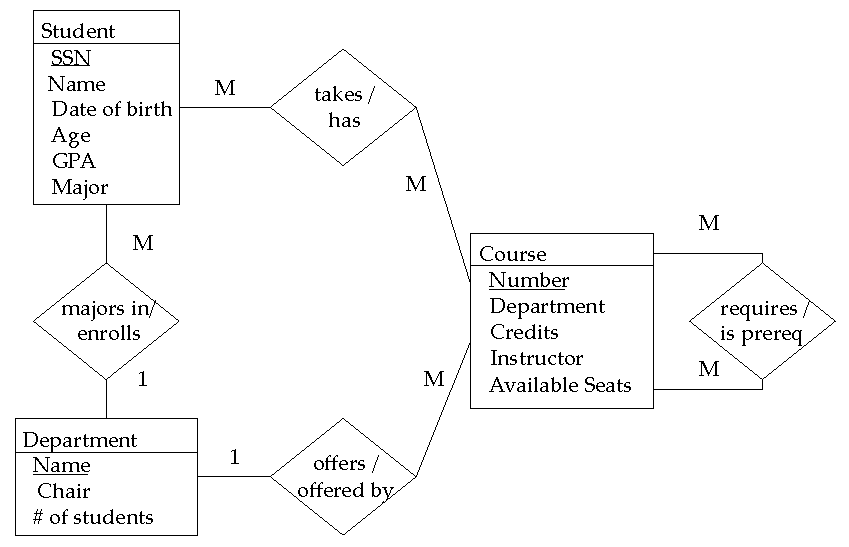
\includegraphics[width=4.5in,height=3.1in]{./image7} \\
\end{tabular}
\end{table}

The ERD allows for an easy interpretation of the relationships between
entities as well as their attributes. Although beyond the scope of the
discussion here, the ERD is a formal language that can be used to
automatically generate the database structure. The relationships in the
ERD allow queries to be asked of the resulting database. For example,
the college could derive a student's course schedule from the database
from the relationship between Student and Course.

\section{The Unified Modeling Language}
\label{section:the-unified-modeling-language}

The \emph{\textbf{Unified Modeling Language}} (UML) was created to
capture the best practices of the object-oriented software development
process. However, it has valuable modeling tools that can be applied
more generally to ECE systems. The objective of this section is to
provide an overview of UML and the six different system views that it
encompasses. A caveat for the reader---UML is complex, and complete
coverage is beyond the scope of this book. In order to fully understand
its subtleties and nuances, the reader is advised to consult the
references provided in Section 6.8.

In order to aid in the explanation of the different views we will create
a UML model of a system called the Virtual Grocer, or v-Grocer for
short. The v-Grocer enables a user to order groceries from home and have
them delivered. The concept is to provide users with a barcode scanner
that is connected to their home computer along with application
software. When the user runs out of an item, he/she scans in the
Universal Product Code (UPC). When users want to order groceries, they
connect to the Internet, log into the grocery store web server, enter
the quantity for the scanned items, and place their order. Once the
order is completed, they are billed and the groceries are delivered to
their houses at a prearranged time.

\subsection{Static View}
\label{subsection:static-view}

Object-oriented design (OOD) is fundamentally different from functional
software design in that it emphasizes objects instead of functions.
\emph{\textbf{Objects}} represent both data (attributes) and the methods
(functions) that can act upon the data. An object represents a
particular instance of something known as a \emph{\textbf{class}}, which
defines the attributes and methods. An object encapsulates all of this
information. The data and methods that an object encapsulates are
available only to that object by default. Thus, other objects cannot
change that state of an object unless given specific permission to do
so. This improves the reliability and maintainability of software
systems, because changes made to the internal representation of a class
are not seen by methods outside of the class.

The intention of the \emph{\textbf{static view}} is to show the classes
in a system and their relationships. The static view is characterized by
a \emph{class diagram}. A very simple class diagram with a single class
is shown in Figure~\ref{figure:classDiagram}. 
The specification of a class has three parts, a
name, a list of attributes, and a set of methods. The name of the class
for this example is Customer and it has three attributes: Name, Address,
and CustId. It has one method associated with it, ChangeAddr(), which
can change the Address attribute. A class, just like an entity in an
ERD, is a generalization of a set of a particular thing or instance. For
example, the Customer class could have a particular instance called Ms.
Robinson.

\begin{figure}
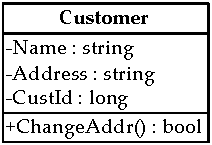
\includegraphics[width=1.2in,height=0.81in]{./image8}
\caption{Class diagram notation. The class has a label
(Customer), attributes (Name, Address, and CustId), and methods
(ChangeAddr()).}
\label{figure:classDiagram}
\end{figure}

Classes are related to one another by relationships that define how
classes interact with each other. For example, if a class is a subset of
another class (a kind of relation) then the subclass inherits all the
attributes and methods of the \emph{superclass}. In UML, there are a
host of relationships; among these are generalization, composition, and
associations. Two classes are related by a \emph{generalization
relationship} when one is a subset of the other. Two classes are related
by a \emph{composition relationship} when one is composed of members of
the other. Two classes are related by an \emph{association relationship}
whenever they need to send messages to one another. Relationships are
drawn as lines connecting the two participant classes. The terminals of
the line have different shapes depending on the type of relationship.
Just like an ERD, the relationships between classes have cardinality
defined by the rule base. In order to illustrate these points, 
Figure~\ref{figure:classVgrocer} 
shows the class diagram for a portion of the v-Grocer system.

\begin{figure}

\includegraphics[width=3.56in,height=2.6in]{./image9}
\caption{Class diagram for the v-Grocer.}
\label{figure:classVgrocer}
\end{figure}

The class diagram has five classes---Customer, Delivery, Order, Item,
and GroceryCart. The GroceryCart class is derived from the many-to-many
relationship which exists between the Order and Item classes. Just like
the rules for an ERD, the cardinality of a relationship is read at the
end of the association in which it is involved. The only difference is
that the many cardinality in a class diagram is denoted by a * symbol.
For example, a delivery is sent to one customer, while a customer may
receive many deliveries.

\subsection{Use-Case View}
\label{subsection:use-case-view}

The intention of the \emph{\textbf{use-case view}} is to capture the
overall behavior of the system from the user's point of view and to
describe cases in which the system will be used. It is characterized by
a \emph{use-case diagram}, and an example for the v-Grocer is shown in
Figure~\ref{figure:useCaseVgrocer}. 
There are only two symbols employed in a use-case diagram,
actors and use-cases. Actors, drawn as stick figure people, are
idealized people or systems that interact with the system. For this
example the actors are customers, delivery people, the database, clerks,
and the web server. Use-cases are drawn as ovals in the diagram, and in
this example, they are WebOrder, DeliverOrder, and AssembleOrder. A
use-case is a particular situation when actors use the system and is
usually represented by a sequence of actions that will be performed by
the system. This sequence of actions typically represents a high level
of functionality. Every actor that interacts with a particular use-case
is connected to it with a line. Finally, the entire collection of
use-cases is enclosed in a rectangle with the actors outside. This
rectangle represents the system boundary and consequently is labeled
with the name of the system.

\begin{figure}
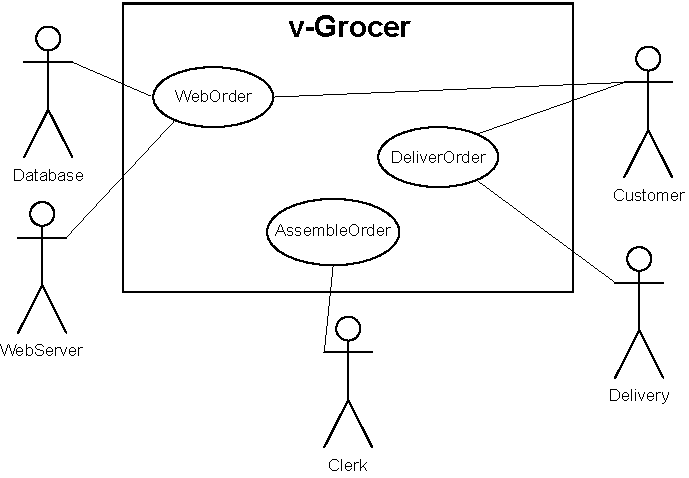
\includegraphics[width=3.9in,height=2.7in]{./image10}
\caption{Use-case diagram for the v-Grocer.}
\label{figure:useCaseVgrocer}
\end{figure}

From Figure~\ref{figure:useCaseVgrocer}
it is apparent that a Customer, the WebServer, and
Database interact when creating a WebOrder. Use-cases are often
described in a table as shown for this particular example in 
Table~\ref{table:webOrderUseCase}.

\textbf{Table 6.3} 


\begin{table}
\caption{WebOrder use-case description.}
\label{table:webOrderUseCase}
\begin{tabular}{|l|m{10cm}|}
\hline
\textbf{Use-Case} & WebOrder \\ \hline
\textbf{Actors} & Customer, Database, and WebServer \\ \hline
\textbf{Description} & This use-case occurs when a customer submits an
order via the WebServer. If it is a new customer, the WebServer prompts
them to establish an account and their customer information is stored in
the Database as a new entry. If they are an existing customer, they have
the opportunity to update their personal information. \\ \hline
\textbf{Stimulus} & Customer order via the GroceryCart. \\ \hline
\textbf{Response} & Verify payment, availability of order items, and if
successful trigger the AssembleOrder use-case. \\ \hline
\end{tabular}
\end{table}

Use-cases focus on a very high level of functionality and describe who
will interact with the system and how they will interact. Given their
high level of abstraction, they can easily be incorporated into a
variety of ECE projects. They are also simple and easy to understand and
thus can be incorporated into presentations to non-technical audiences.
Finally, use-cases are simply not busy work---they are fundamental to
the development of other UML models.

\subsection{State Machine View}
\label{subsection:state-machine-view}

The \emph{\textbf{state machine}} \emph{\textbf{view}} is characterized
by a \emph{state diagram} as was discussed in Section 6.2. Again, the
intention of a state diagram is to describe systems with memory. 
Figure~\ref{figure:stateDiagramVgrocer} shows the state 
view of a customer logging into the v-Grocer web
server.


\begin{figure}
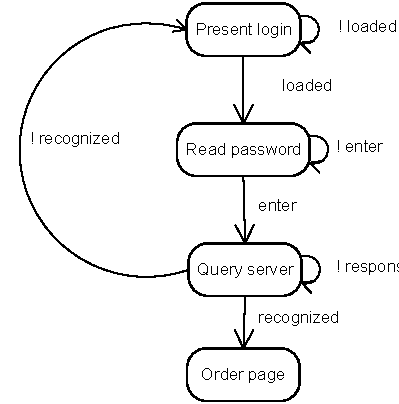
\includegraphics[width=2in,height=2.in]{./image11}
\caption{State diagram for the v-Grocer customer login.}
\label{figure:stateDiagramVgrocer}
\end{figure}

\subsection{Activity View}
\label{subsection:activity-view}

The intention of the \emph{\textbf{activity view}}, characterized by an
\emph{activity diagram}, is to describe the sequencing of processes
required to complete a task. In UML, the tasks elaborated are the
individual use-cases identified in a use-case diagram. Since more than
one actor may be involved in completing a task, an activity diagram can
express the concurrent nature of tasks. An activity diagram is composed
of states, transitions, forks, and joins. 
Figure~\ref{figure:activityDiagramVgrocer} contains an
activity diagram for the v-Grocer order delivery system. The diagram
gives a clear visual picture for the activities that need to be
completed for an order to be packed and delivered. After a complete
order is placed, the flow is forked into two concurrent processing
branches. One of these branches is for completion of the order, while
the other addresses its scheduling, delivery, and coordination with
other deliveries. When both of those processes are completed, they are
joined together and then the delivery run is made.


\begin{figure}

\includegraphics[width=5.5in,height=0.9in]{./image12}
\caption{Activity diagram for order processing and delivery
for the v-Grocer.}
\label{figure:activityDiagramVgrocer}
\end{figure}

\subsection{Interaction View}
\label{subsection:interaction-view}

The intention of the \emph{\textbf{interaction view}} is to show the
interaction between objects. It is characterized by collaboration and
sequence diagrams. In an object-oriented system, tasks are completed by
passing messages between objects. The interaction view shows how
messages are exchanged in order to accomplish a task. These tasks are
usually the use-cases. Since messages are sent through time, the
interaction view must be able to express the concept of order. We start
by examining collaboration diagrams.

Two objects collaborate together in order to produce some meaningful
result. A \emph{collaboration diagram} shows the sequencing of messages
that are exchanged between classes in order to complete a task. It
consists of the classes that participate in the realization of the task
and the messages exchanged. The messages are drawn as arrows from the
sending object to the receiving object. The message arrows are labeled
with the name of the message and its numerical position in the sequence
of messages exchanged to realize the task. For example, 
Figure~\ref{figure:collaborationDiagramWebOrder}
shows how the WebOrder use-case is realized using the Customer,
WebServer, and Database classes. Note, WebServer and Database are
introduced as new classes and are not shown as part of the class diagram
in Figure 6.9.

\begin{figure}

\includegraphics[width=4in,height=1.17in]{./image13}
\caption{Collaboration diagram for the WebOrder use-case.}
\label{figure:collaborationDiagramWebOrder}
\end{figure}


The collaboration diagram is similar in form to the class diagram, the
difference being that the relationships are annotated with the messages
that are exchanged. Consequently, the collaboration diagram aides the
developers in understanding and implementing the methods used between
classes. In order to emphasize the order in which messages are
exchanged, a developer can also use a sequence diagram.

A \emph{sequence diagram} contains the same information as the
corresponding collaboration diagram. Where the collaboration diagram
emphasizes the objects that interact to produce a behavior, a sequence
diagram emphasizes the message order that produces a behavior. As shown
in Figure~\ref{figure:sequenceDiagramWebOrder}, 
the classes that participate in the behavior are listed
in a row at the top of the diagram. From each class a dotted vertical
line is drawn downward that represents the lifeline of its class (the
vertical axis represents time). When an object is actively requesting or
waiting for information from another object, a rectangle is drawn over
the dotted lifeline of the object. The message is drawn as an arrow from
the sending object to the receiving object and labeled with the name of
the message. The activity diagrams can be applied generally to ECE
systems to show the interaction between entities, particularly the
sequencing of messages.

\begin{figure}
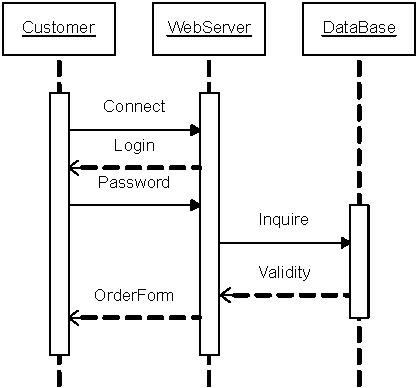
\includegraphics[width=2.6in,height=2.4in]{./image14}
\caption{Sequence diagram for the WebOrder use-case.}
\label{figure:sequenceDiagramWebOrder}
\end{figure}

\subsection{Physical View}
\label{subsection:physical-view}

The intention of the \emph{\textbf{physical view}} is to demonstrate the
physical components of the system and how the logical views map to them.
The physical view is characterized by a component and deployment
diagram. A \emph{component diagram} shows the software files and the
interrelationships that make up the system. Software files are shown in
rectangles. Lines connect together files that need to communicate. A
\emph{deployment diagram} shows the hardware and communications
components that will be used to realize the system. The hardware
components are drawn as cubes and labeled with their names. 
Figure~\ref{figure:vGrocerSystem}
shows a combined component and deployment diagram for the v-Grocer
system. The software files are the Browser, v-Grocer, Apache, and
Oracle, while the hardware components are the Customer, WebServer, and
Database.

\begin{figure}
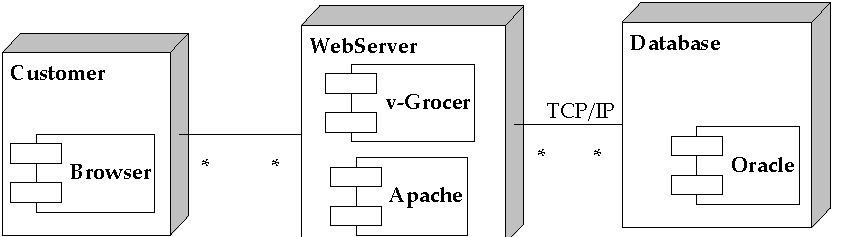
\includegraphics[width=4.8in,height=1.4in]{./image15}
\caption{The combined component and deployment diagram for
the v-Grocer. The software files are the Browser, v-Grocer, Apache, and
Oracle, while the hardware components are the Customer, WebServer, and
Database.}
\label{figure:vGrocerSystem}
\end{figure}


\section{Project Application: Selecting Models}
\label{section:project-application-selecting-models}

Chapters 5 and 6 have presented a variety of models for representing the
behavior of systems. The design team needs to select the correct
combination of tools to properly describe a design for its eventual
implementation. Table 6.4 provides a summary of the models and their
different intentions.

Table 6.4

\begin{table}
\caption{Guidance for model selection.}
\label{table:<context>}
\begin{tabular}{|l|m{10cm}|}
\hline
\textbf{Model} & \textbf{Intention} \\ \hline
\textbf{Functional Decomposition} & To describe the input, output, and
functional transformations applied to information (electrical signals,
bits, energy, etc.) in a system. It is broad in application. This often
provides a view that is close to the actual system implementation. See
Chapter 5. \\ \hline
\textbf{State Diagram} & To describe the behavior of systems with
memory. They are very flexible when it comes to application. They are
often applied to digital design, but state diagrams can also be used to
describe the high level behavior of complex systems. The only
prerequisite on their use is that the system has memory. See Section
6.2. \\ \hline
\textbf{Flowchart} & To describe a process or algorithm, including its
steps and control. They are applicable to many problem domains from
software to describing business practices. See Section 6.3. \\ \hline
\textbf{Data Flow Diagram} & To model the processing, transformation, and flow of
data inside a system. They are typically supplemented by an event table
describing all possible events and the resulting actions. Creating a DFD
requires the designer to carefully think about the uses of the system
and how the system is to react to external users and events. See Section
6.4. \\  \hline
\textbf{Entity Relationship Diagram} & To catalog a set of related objects (entities), their
attributes, and the relationships between them. ERDs capture the
entities and relationships of a portion of the world into a formal data
model. The graphical language describes the attributes of the entities
and the cardinality of the relationships. ERDs are formal enough to be
unambiguously translated into a complete description of a database
system. See Section 6.5. \\  \hline
\textbf{The Unified Modeling Language.} & The intention of UML is to
describe complex software systems. However, certain views are well
suited to describing systems at a high level and are applicable to many
domains. The process of viewing a system from the six perspectives
listed below decreases the chances that crucial details of the design
will be overlooked. \\  \hline
\textbf{Class Diagram} & To describe classes and their relationship in
an object-oriented software system. Class diagrams are primarily for
software design and are not easily accessible to a non-technical
audience. See Section 6.6.1. \\ \hline
\textbf{Use-Case Diagram} &  To capture the overall behavior of the system from
the user's point of view and describe cases in which the system will be
used. See Section 6.6.2. \\  \hline
\textbf{State Machine} & This is essentially the same as the state
diagram, but is also a formal UML view. See Sections 6.2 and 6.6.3. \\  \hline
\textbf{Activity Diagram} &  To describe the sequencing of processes required to
complete a task. Composed of states, transitions, forks, and joins. Can
show concurrent processes. See Section 6.6.4. \\  \hline
\textbf{Interaction Diagram} & To show the interaction and passing of messages
between entities in a system. Characterized by both collaboration and
sequence diagrams. See Section 6.6.5. \\  \hline
\textbf{Physical Diagram} &  To describe the arrangement and connections of the
physical components that constitute a system. In the case of UML, it is
characterized by a component and deployment diagram. See Section
6.6.6. \\  \hline
\end{tabular}
\end{table}

\section{Summary and Further Reading}
\label{section:summary-and-further-reading}

Models provide a convenient method of describing a system at a high
level of abstraction. This allows a system to be described without
having to determine all of the implementation details. All models are
not the same---they come in a variety of forms and each is designed to
serve a different intention. The properties of effective models were
presented, and we saw that they are similar to those of an engineering
requirement. Models should encourage innovation by allowing the
exploration of alternative implementations. Since models are built from
abstractions of the actual system components, they are an effective
means for communicating with non-technical stakeholders. Finally, models
provide an excellent means of documenting the development of a design
from the highest level down to the detailed design.

This chapter presented a variety of models for describing system
behavior that included state diagrams, flowcharts, data flow diagrams,
entity relationship diagrams, and the Unified Modeling Language. Table
6.4 provides a quick reference that describes the intention and
application of the models examined in both Chapters 5 and 6.

Flowcharts have been around for quite some time and an early work
describing them is \ul{Flowcharts} by Chapin {[}Cha71{]}. The book
\ul{Programming Logic and Design} {[}Far02{]} covers flowcharts
extensively and their application in programming. State diagrams are
fundamental to the ECE field and further information on them is
available in virtually any introductory digital design textbook. Data
flow diagrams and entity relationship diagrams are common tools used in
information systems analysis and design and can be further explored in
\ul{Systems Analysis and Design} {[}Sat02{]} and \ul{Fundamentals of
Database Systems} {[}Elm94{]}. Two references for UML are \ul{The
Unified Modeling Language Reference Manual} {[}Rum98{]} and \ul{Schaum's
Outline of UML} {[}Ben01{]}.
